\section{General system description}

The algorithms implemented in this thesis used the C++ programming
language. The overall architecture of the system is the following:

\begin{figure}

  \centering

  \begin{tikzpicture}
    \node[module]                        (I0) {\tiny Input};
    \node[module, right=3mm of I0]       (I1) {\tiny Parser (Z3)};
    \node[module, right=3mm of I1]       (I2) {\tiny Preprocessor};
    \node[module, right=23mm of I2]      (I4) {\tiny Sat engine (PicoSAT/TraceCheck)};
    \node[module, above=2mm of I4]       (I3) {\tiny Theory Combination Interpolator};
    \node[module, below left=3mm of I4]  (I5) {\tiny EUF interpolator};
    \node[module, below right=3mm of I4] (I6) {\tiny UTVPI interpolator};
    \node[module, right=24mm of I4] (I7) {\tiny Output};
    \foreach \i in {5, 6}
    \draw[<->, dashed] (I4)--(I\i);
    \node[fit=(I4) (I5) (I6), draw, inner sep=0.5mm]           (fitThCombInternal) {};
    \node[fit=(I3) (fitThCombInternal), draw, inner sep=0.5mm] (fitThComb)         {};
    \draw[->] (I0)--(I1);
    \draw[->] (I1)--(I2);
    \draw[->] (I2)--(I4);
    \draw[->] (I2)--(I4);
    \draw[->] (I4)--(I7);
  \end{tikzpicture}

  \caption{General System Diagram} \label{general_architecture}

\end{figure}

%%% Local Variables:
%%% mode: latex
%%% TeX-master: "main"
%%% End:

\begin{figure}

  \centering

  \begin{tikzpicture}
    \node[module]                        (I0) {\tiny Input};
    \node[module, right=3mm of I0]       (I1) {\tiny Parser (Z3)};
    \node[module, right=3mm of I1]       (I9) {\tiny Preprocessor};
    \node[module, right=3mm of I9]       (I8) {\tiny Congruence closure};
    \node[module, right=3mm of I8]       (I4) {\tiny Horn clause generator};
    \node[module, above=2mm of I4]       (I3) {\tiny EUF Interpolator};
    \node[module, below=5mm of I4, text width=20mm]  (I5) {\tiny Congruence closure with explanations};
    \node[module, below right=3mm of I4] (I6) {\tiny Simplifier (Z3)};
    \node[module, right=24mm of I4] (I7) {\tiny Output};
    \draw[->, dashed] (I4)--(I5);
    \draw[->, dashed] (I4)--(I6);
    \node[fit=(I8) (I4) (I5) (I6), draw, inner sep=0.5mm]           (fitThCombInternal) {};
    \node[fit=(I3) (fitThCombInternal), draw, inner sep=0.5mm] (fitThComb)         {};
    \draw[->] (I0)--(I1);
    \draw[->] (I1)--(I9);
    \draw[->] (I9)--(I8);
    \draw[->] (I8)--(I4);
    \draw[->] (I5)--(I4);
    \draw[->] (I6)--(I7);
  \end{tikzpicture}

  \caption{EUF Interpolator Diagram} \label{euf_architecture}

\end{figure}

%%% Local Variables:
%%% mode: latex
%%% TeX-master: "main"
%%% End:

\begin{figure}

  \centering

  \begin{tikzpicture}
    \node[module]                        (I0) {\tiny Input};
    \node[module, right=3mm of I0]       (I1) {\tiny Parser (Z3)};
    \node[module, right=3mm of I1]       (I9) {\tiny Preprocessor};
    \node[module, right=3mm of I9]       (I8) {\tiny Indexing table};
    \node[module, right=3mm of I8]       (I4) {\tiny Matching and Variable elimination};
    \node[module, above=2mm of I4]       (I3) {\tiny UTVPI Interpolator};
    \node[module, below=3mm of I4] (I6) {\tiny Simplifier};
    \node[module, right=3mm of I4] (I7) {\tiny Output};
    \draw[->, dashed] (I4)--(I6);
    \node[fit=(I8) (I4) (I6), draw, inner sep=0.5mm]           (fitThCombInternal) {};
    \node[fit=(I3) (fitThCombInternal), draw, inner sep=0.5mm] (fitThComb)         {};
    \draw[->] (I0)--(I1);
    \draw[->] (I1)--(I9);
    \draw[->] (I9)--(I8);
    \draw[->] (I8)--(I4);
    \draw[->] (I6)--(I7);
  \end{tikzpicture}

  \caption{UTVPI Interpolator Diagram} \label{utvpi_architecture}

\end{figure}

%%% Local Variables:
%%% mode: latex
%%% TeX-master: "main"
%%% End:


All the decision procedures mentioned in this chapter
were implemented with the exception of the SAT/SMT algorithms.
For the latter, zChaff \cite{935565} and Z3 
\cite{10.1007/978-3-540-78800-3_24} were chosen as the 
libraries to work with these algorithms. 
The rest of this section discusses some minor modifications 
implemented in the above mentioned Z3 and zChaff libraries.

\subsection{Minor modifications to Z3}

Z3 standard input is SMTLib2 \cite{BarFT-SMTLIB}. This grammar
does not provide a standard specification regarding a suitable
format to work with interpolants. Interpolation software
read interpolant formulas based on the order of appereance
in a conjunction \cite{mcmillan2011interpolants}. In our case
we require two conjuncts of conjunctions of literals in the
EUF theory, UTVPI theory or combined theory. 

As we can notice in figures \ref{general_architecture}, \ref{euf_architecture},
and \ref{utvpi_architecture}, there is preprocessor component which prefixes
the names of uninterpreted symbols with the strings a\_, b\_, c\_
to indicate that the symbol name is either an A-local, B-local, or
common symbol respectively. We extended Z3's API with functions
that test if a formula is A-local, B-local, AB-pure, AB-common
based of the definitions in \cite{10.1007/11532231_26} because 
it is necessary to constantly check this conditions for splitting
purposes. Another reason for the latter is justified because the 
implemented congruence closure algorithm takes as an additional
criteria to maintain as representative term an AB-common term.
A similar change was implemented in the congruence closure implementation
of Z3. Nonetheless, it was irrelevant since Z3's internal structure
separates the abstract syntax tree, which is part of its API
with the enode data structures, which does not allow the super
to modify it. This is the reason why it was not
possible to work directly with Z3 congruence closure implementation
and a separate implementation was necessary.

\subsection{Minor modifications to zChaff}

We used zChaff to reconstruct a resolution-based proof necessary 
for Pudlak's algorithm in the interpolation combination componente. 
Given that Z3 provides a user friendly proof-producing API
\cite{Moura_proofsand}, why did the implementation
work require another SAT solver to obtain the resolution-proof?

There are several reasons for the latter. First, the author of the
thesis was not able to find an appropriate configuration of parameters
for the SMT solver to provide such proofs. In order to grasp an idea
of the latter, it was implemented a Z3 proof parser that render
a pdf rendered by \LaTeX. Many examples indicated that
Z3 selects more convenient theories to work with some problems. For
instance, the formula in pure propositional logic shown in figure 
\ref{query_proof_problem} used proof rules from EUF \footnote{Z3 uses
the term monotonicity instead of congruence}.

\begin{figure}
  \centering
  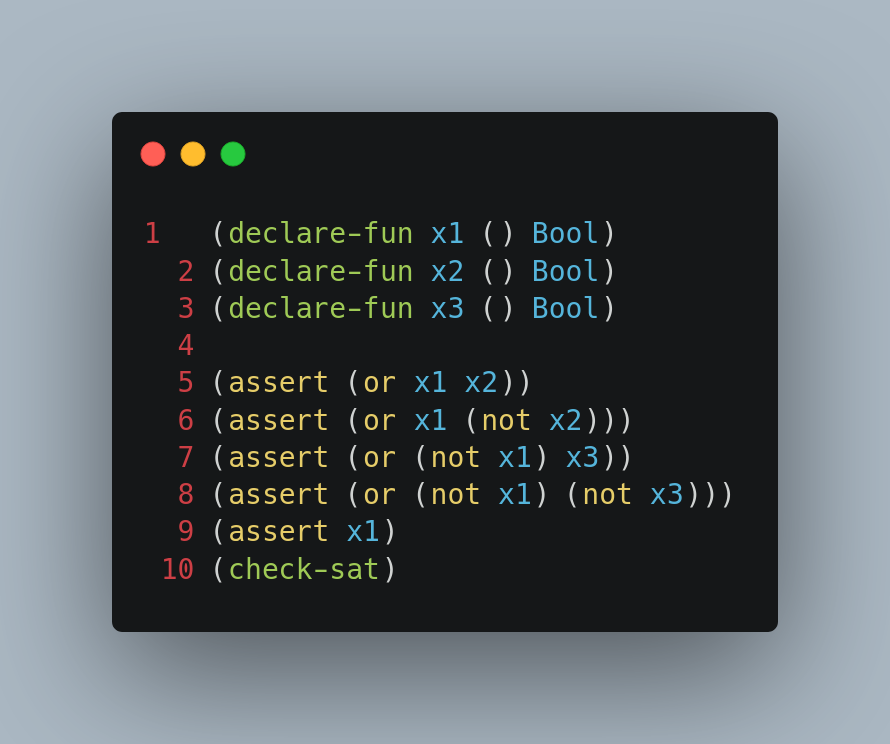
\includegraphics[scale=0.2]{query_screenshot}
  \caption{Problematic SMT query for resolution proofs} \label{query_proof_problem}
\end{figure}


%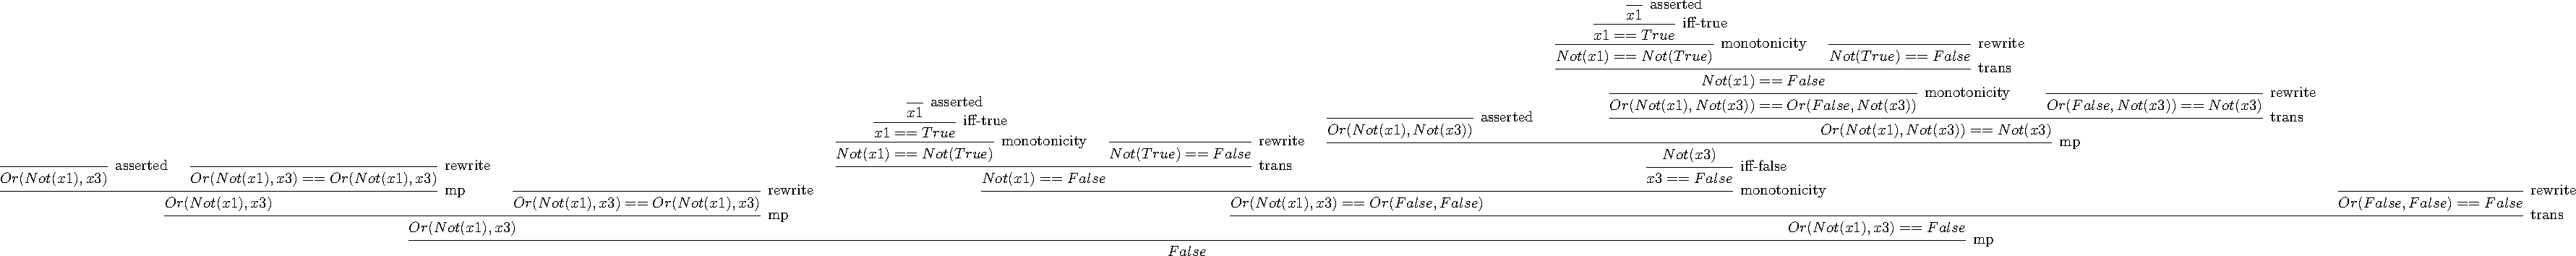
\includepdf[scale=0.2,pages=-,pagecommand={},width=\textwidth, angle=90]{python_proof.pdf}
\begin{figure}
  %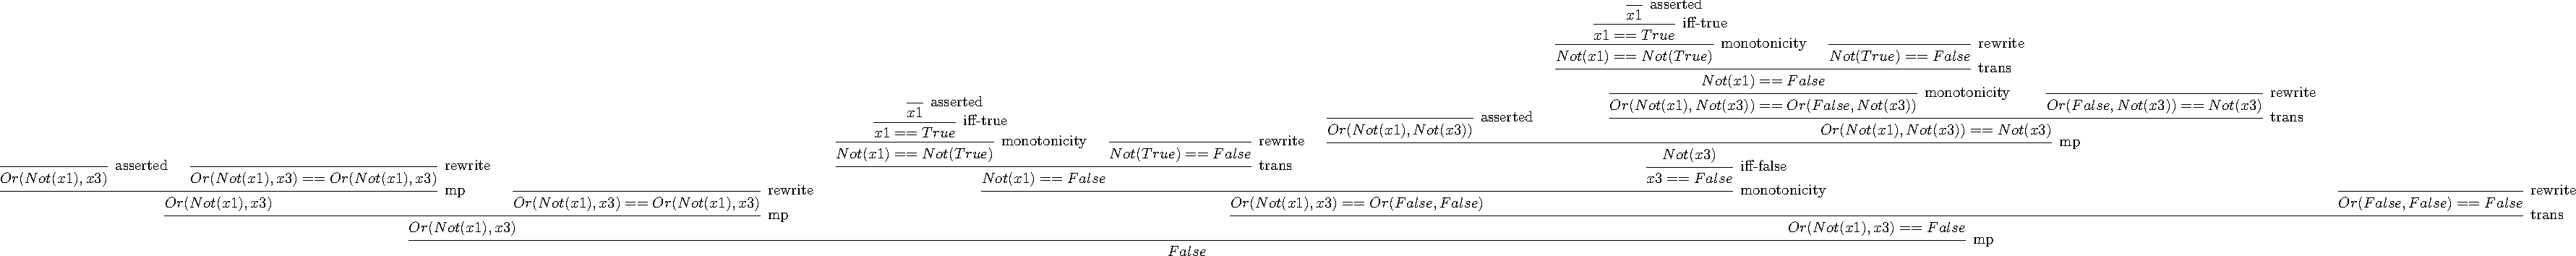
\includepdf[scale=0.8,pages=-,angle=0]{python_proof.pdf}
  \begin{turn}{0}
\resizebox{420}{40}
{
  \centering
  \begin{prooftree}[separation=-0.5em]\infer0[asserted]{Or(Not(x1), x3)}\infer0[rewrite]{Or(Not(x1), x3)==Or(Not(x1), x3)}\infer2[mp]{Or(Not(x1), x3)}\infer0[rewrite]{Or(Not(x1), x3)==Or(Not(x1), x3)}\infer2[mp]{Or(Not(x1), x3)}\infer0[asserted]{x1}\infer1[iff-true]{x1==True}\infer1[monotonicity]{Not(x1)==Not(True)}\infer0[rewrite]{Not(True)==False}\infer2[trans]{Not(x1)==False}\infer0[asserted]{Or(Not(x1), Not(x3))}\infer0[asserted]{x1}\infer1[iff-true]{x1==True}\infer1[monotonicity]{Not(x1)==Not(True)}\infer0[rewrite]{Not(True)==False}\infer2[trans]{Not(x1)==False}\infer1[monotonicity]{Or(Not(x1), Not(x3))==Or(False, Not(x3))}\infer0[rewrite]{Or(False, Not(x3))==Not(x3)}\infer2[trans]{Or(Not(x1), Not(x3))==Not(x3)}\infer2[mp]{Not(x3)}\infer1[iff-false]{x3==False}\infer2[monotonicity]{Or(Not(x1), x3)==Or(False, False)}\infer0[rewrite]{Or(False, False)==False}\infer2[trans]{Or(Not(x1), x3)==False}\infer2[mp]{False}\end{prooftree}
}
\end{turn}

%%% Local Variables:
%%% mode: latex
%%% TeX-master: "main"
%%% End:

  \caption{Z3 proof of figure \ref{query_proof_problem}} \label{smt_proof_problem}
\end{figure}


Thus, we opted to use the zChaff SAT solver which implements the DPLL algorithm. 
The minor modifications to the software was to include the pivots 
in the proof trace zChaff produces. Many SAT solvers produce more sophisticated 
proofs in formats like DRAT, DRUP, etc. The latter require to implement unit-propagation
to construct a resolution-base proof and hence the implementation might unintentionally
slow the performance of the solver during the proof-checking step.

%%% Local Variables:
%%% mode: latex
%%% TeX-master: "main"
%%% End:
